\section{Бинаризация признаков}

Бинаризация признаков – это процесс преобразования исходных признаков в бинарные переменные, которые принимают значения \(0\) или \(1\). 
%Этот метод широко используется в задачах %машинного обучения, особенно в логических %методах классификации, где входные данные %должны быть представлены в виде набора %булевых предикатов.

\subsection{Бинаризация количественных признаков}

Для признака \( f: X \to D_f \), где \( D_f \) – множество возможных значений признака, бинаризация заключается в создании предикатов, проверяющих выполнение определённых условий. Эти предикаты позволяют разбить множество значений признака на подмножества, которые можно использовать в логических моделях.

В зависимости от типа признака, бинаризация осуществляется следующим образом:
\begin{itemize}
    \item \textbf{Номинальный признак} (\(f\) принимает конечное множество значений, без упорядоченности):
    \[
    \beta(x) = [f(x) = d], \quad d \in D_f;
    \]
    \[
    \beta(x) = [f(x) \in D'], \quad D' \subset D_f.
    \]
    \item \textbf{Порядковый или количественный признак} (\(f\) принимает значения, между которыми можно определить порядок):
    \[
    \beta(x) = [f(x) \leq d], \quad d \in D_f;
    \]
    \[
    \beta(x) = [d \leq f(x) \leq d'], \quad d, d' \in D_f, \, d < d'.
    \]
\end{itemize}

Для количественных признаков (\(f: X \to \mathbb{R}\)) важно выбирать такие пороговые значения \(d\), которые разделяют выборку на значимые группы. Например, 
%пороги \(d\) могут быть определены как средние значения между %соседними элементами вариационного ряда \(f(x_1), \dots, %f(x_\ell)\), упорядоченного по возрастанию:
\[
d_i = \frac{f^{(i)} + f^{(i+1)}}{2}, \quad f^{(i)} \neq f^{(i+1)}, \; i = 1, \dots, \ell - 1,
\]
где \(f^{(1)} \leq f^{(2)} \leq \dots \leq f^{(\ell)}\) – упорядоченные значения признака. (См. рис)

Такими способами можно получить много разных предикатов. Мы хотим выбрать из них самые ''лучшие'' (в каком-либо смысле). Для этого разобьем диапазон значений признака на зоны.

\begin{figure}
    \centering
    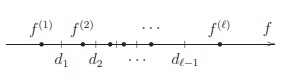
\includegraphics[scale = 1]{images/bin1.png}
    \caption{Вариационный ряд значений признака $f(x)$ и пороги $d_i$}
\end{figure}

\subsection{Разбиение диапазона значений признака на зоны}

Каждая зона определяется бинарным предикатом:
\begin{align*}
\zeta_0(x) &= [f(x) < d_1], \\
\zeta_s(x) &= [d_s \leq f(x) < d_{s+1}], \quad s = 1, \dots, r-1, \\
\zeta_r(x) &= [d_r \leq f(x)].
\end{align*}

Способы разбиения:
\begin{itemize}
    \item Жадная максимизация информативности путем слияний
    \item Разбиение на равномощные подвыборки
    \item Разбиение по равномерной сетке ''удобных'' значений (например, с минимальным числом значащих цифр)
    \item Объединение нескольких разбиений
\end{itemize}

\subsection{Жадный алгоритм слияния зон}

Алгоритм начинает с разбиения на ''мелкие'' зоны. Пороги проходят между всеми соседними парами точек, принадлежащих \emph{разным} классам, т.~к. расстановка порогов между точками одного класса приведет только к уменьшению информативности зон. Далее зоны укрупняются путём слияния \emph{троек} соседних зон. Зоны сливаются до тех пор, пока
информативность некоторой слитой зоны превышает информативность
исходных зон, либо пока не будет получено заданное количество зон $r$. Каждый раз сливается тройка, дающая наибольший выигрыш в информативности.

\begin{figure}
    \centering
    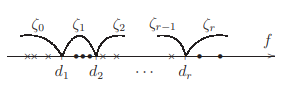
\includegraphics[scale = 1]{images/bin2.png}
    \caption{Начальное разбиение на зоны}
\end{figure}

\newpage
\textbf{Вход:}
\begin{itemize}
    \item $f(x)$ — признак;
    \item $c \in Y$ — выделенный класс;
    \item $X^\ell = \{(x_i, y_i)\}_{i=1}^\ell$ — выборка, упорядоченная по возрастанию $f(x_i)$;
    \item $r$ — желаемое количество зон;
    \item $\delta_0$ — порог слияния зон (по умолчанию $\delta_0 = 0$).
\end{itemize}

\textbf{Выход:}
\[
D = \{d_1, \dots, d_n\} \text{ — строго возрастающая последовательность порогов;}
\]

\hline

\begin{enumerate}
    \item $D := \emptyset;$
    \item \textbf{для всех} $i = 2, \dots, \ell$:
    \begin{itemize}
        \item \textbf{если} $f(x_{i-1}) \neq f(x_i)$ и $[y_{i-1} = c] \neq [y_i = c]$ \textbf{то}
        \begin{itemize}
            \item добавить новый порог $d := \frac{f(x_{i-1}) + f(x_i)}{2}$ в конец последовательности $D$;
        \end{itemize}
    \end{itemize}
    \item \textbf{повторять}
    \begin{enumerate}
        \item \textbf{для всех} $d_i \in D, i = 1, \dots, |D| - 1$:
        \begin{itemize}
            \item вычислить выигрыш от слияния тройки соседних зон $\zeta_{i-1}, \zeta_i, \zeta_{i+1}$:
            \[
            \delta_i := I_c(\zeta_{i-1} \cup \zeta_i \cup \zeta_{i+1}) - \max\{I_c(\zeta_{i-1}), I_c(\zeta_i), I_c(\zeta_{i+1})\};
            \]
        \end{itemize}
        \item найти тройку зон, для которой слияние наиболее выгодно:
        \[
        i := \arg \max \delta_i;
        \]
        \item \textbf{если} $\delta_i > \delta_0$ \textbf{то}
        \begin{itemize}
            \item слить зоны $\zeta_{i-1}, \zeta_i, \zeta_{i+1}$, удалить пороги $d_i$ и $d_{i+1}$ из последовательности $D$;
        \end{itemize}
    \end{enumerate}
    \item \textbf{пока} $|D| > r + 1$.
\end{enumerate}

\subsection{Задачи}

\textbf{Задача 1}
Предположим, вы владелец интернет-магазина, и у вас есть данные о стоимости товаров и их популярности (популярен — \( 1 \), непопулярен — \( 0 \)). 
Для анализа спроса вы хотите разбить товары на ценовые зоны, чтобы лучше понять поведение покупателей.

Данные представлены в таблице:

\[
\begin{array}{|c|c|c|}
\hline
\text{№ товара} & \text{Цена товара (\$)} & \text{Популярность } y \\
\hline
1 & 10 & 1 \\
2 & 12 & 1 \\
3 & 15 & 0 \\
4 & 17 & 1 \\
5 & 20 & 0 \\
6 & 23 & 0 \\
7 & 25 & 1 \\
\hline
\end{array}
\]

Как алгоритм слияния зон первично разобьёт выборку на ценовые зоны?

\textbf{Решение}
Рассчитаем пороги:

\[
\begin{aligned}
&d_1 = \frac{12 + 15}{2} = 13.5, \\
&d_2 = \frac{15 + 17}{2} = 16.0, \\
&d_3 = \frac{17 + 20}{2} = 18.5, \\
&d_4 = \frac{23 + 25}{2} = 24.0
\end{aligned}
\]

На основе рассчитанных порогов получаем зоны:

\[
\begin{aligned}
&\zeta_0(x) = [\text{Цена} < 13.5], \\
&\zeta_1(x) = [13.5 \leq \text{Цена} < 16.0], \\
&\zeta_2(x) = [16.0 \leq \text{Цена} < 18.5], \\
&\zeta_4(x) = [29.0 \leq \text{Цена} < 24.0], \\
&\zeta_5(x) = [\text{Цена} \geq 24.0].
\end{aligned}
\]

\textbf{Задача 2}
Будут ли разбиения диапазона меняться в зависимости от класса, относительно которого они производятся? Как изменить алгоритм для получения ''универсального'' разбиения, учитывающего сразу все классы? 

\textbf{Решение}
Да, будут, т.~к. информативность зависит от класса. Нужно заменить критерий информативности многоклассовым критерием.

\textbf{Задача 3}
Какую сложность имеет алгоритм слияния зон? Как можно его ускорить?

\textbf{Решение}
Этот алгоритм имеет трудоёмкость $O(l^2)$. Его можно заметно ускорить, если на каждой итерации сливать не одну тройку зон, а $\tau l$ троек с достаточно большим выигрышем $\delta I_i$, при условии, что они не перекрываются. В этом случае трудоёмкость составляет $O(l / \sqrt{\tau})$.

\section{Взвешенное голосование правил}

Допустим, имеется консилиум экспертов, каждый член которого может допустить ошибку. Процедура голосования — это способ повышения качества принимаемых решений, при котором ошибки отдельных экспертов компенсируют друг друга.

Ранее принцип голосования применялся для построения композиций из произвольных алгоритмов классификации. Теперь рассмотрим композиции, состоящие из логических закономерностей.

\subsection{Принцип голосования}

Пусть для каждого класса $c \in Y$ построено множество логических закономерностей (правил), специализирующихся на различении объектов данного класса:

\[
R_c = \{ \varphi_{tc} : X \to \{0, 1\} \mid t = 1, \dots, T_c \}
\]

Считается, что если $\varphi_{tc}(x) = 1$, то правило $\varphi_{tc}$ относит объект $x \in X$ к классу $c$. Если же $\varphi_{tc}(x) = 0$, то правило воздерживается от классификации объекта $x$.

Алгоритм простого голосования (simple voting) подсчитывает долю правил в наборах $R_c$, относящих объект $x$ к каждому из классов:

\[
\Gamma_c(x) = \frac{1}{T_c} \sum_{t=1}^{T_c} \varphi_{tc}(x), \quad c \in Y,
\]

и относит объект $x$ к тому классу, за который подана наибольшая доля голосов:

\[
a(x) = \arg \max_{c \in Y} \Gamma_c(x).
\]

Если максимум достигается одновременно на нескольких классах, выбирается тот, для которого цена ошибки меньше.

Нормирующий множитель $\frac{1}{T_c}$ вводится для того, чтобы наборы с большим числом правил не перетягивали объекты в свой класс.

\subsection{Алгоритм взвешенного голосования}
Алгоритм взвешенного голосования (weighted voting, WV) действует более тонко, учитывая, что правила могут иметь различную ценность. Каждому правилу $\varphi_{tc}$ приписывается вес $\alpha_{tc} \geq 0$, и при голосовании берется взвешенная сумма голосов:

\[
\Gamma_c(x) = \sum_{t=1}^{T_c} \alpha_{tc} \varphi_{tc}(x), \quad \alpha_{tc} > 0.
\]

Веса нормируются на единицу:

\[
\sum_{t=1}^{T_c} \alpha_{tc} = 1, \quad \forall c \in Y.
\]

Поэтому функцию $\Gamma_c(x)$ называют также выпуклой комбинацией правил $\varphi_1, \dots, \varphi_{T_c}$. Очевидно, простое голосование является частным случаем взвешенного, когда веса одинаковы и равны $\frac{1}{T_c}$.

На первый взгляд, вес правила должен определяться его информативностью. Однако, важно также учитывать, насколько данное правило уникально. Если имеется 10 хороших, но одинаковых (или почти одинаковых) правил, их суммарный вес должен быть сравним с весом столь же хорошего правила, не похожего на все остальные. Таким образом, веса должны учитывать не только ценность правил, но и их различность.

Простой общий подход к настройке весов заключается в том, чтобы сначала найти набор правил $\{ \varphi_{tc}(x) \}$, затем принять их за новые (бинарные) признаки и построить в этом новом признаковом пространстве линейную разделяющую поверхность (кусочно-линейную, если $|Y| > 2$). Для этого можно использовать логистическую регрессию, однослойный персептрон или метод опорных векторов. Существуют и другие подходы. Например, в разделе 1.5.4 будет рассмотрен метод бустинга, в котором правила настраиваются последовательно, и для каждого правила сразу вычисляется его вес.

\subsection{Проблема диверсификации правил}
Голосующие правила должны быть существенно различны, иначе они будут бесполезны для классификации. Продолжая аналогию с консилиумом, заметим, что нет никакого смысла держать в консилиуме эксперта A, если он регулярно подсматривает решения у эксперта B.

Приведем простое теоретико-вероятностное обоснование принципа диверсификации, или повышения различности (diversity) правил \cite{14}. Пусть $X$ — вероятностное пространство, множество ответов $Y$ конечно. Введем случайную величину $M(x)$, равную перевесу голосов в пользу правильного класса; её называют также отступом (margin) объекта $x$ от границы классов:

\[
M(x) = \Gamma_c(x) - \Gamma_{\overline{c}}(x), \quad \Gamma_{\overline{c}}(x) = \max_{y \in Y \setminus \{c\}} \Gamma_y(x), \quad c = y^*(x).
\]

Если отступ положителен ($M(x) > 0$), то алгоритм голосования правильно классифицирует объект $x$. Предположим, что в среднем наш алгоритм классифицирует хотя бы немного лучше, чем наугад: $E[M] > 0$. Тогда можно оценить вероятность ошибки по неравенству Чебышева:

\[
P\{M < 0\} \leq P\{|E[M] - M| > E[M]\} \leq \frac{D_M}{(E[M])^2}.
\]

Отсюда вывод: для уменьшения вероятности ошибки необходимо максимизировать ожидание перевеса голосов $E[M]$ и минимизировать его дисперсию $D_M$. Для выполнения этих условий каждый объект должен выделяться примерно одинаковым числом правил. Обычно ни одно из правил не выделяет класс целиком, поэтому правила должны быть существенно различны, то есть выделять существенно различные подмножества объектов.

Неплохая эвристика, усиливающая различия между правилами и позволяющая равномернее выделять объекты обучения, используется в алгоритме CORAL \cite{12}. Сначала для фиксированного класса $c \in Y$ строится покрывающий набор правил точно так, как это делалось для решающих списков. Затем строится второй покрывающий набор, но при этом запрещается использовать признаки, часто входившие в закономерности первого набора. Поэтому второй набор неминуемо окажется отличным от первого. Затем запрещаются признаки, часто входившие в оба набора, и строится третий набор. И так далее, для каждого класса $c \in Y$.

\subsection{Отказы от классификации}
Возможны ситуации, когда ни одно из правил не выделяет классифицируемый объект $x$. Тогда алгоритм должен либо отказываться от классификации, либо относить объект к классу, имеющему наименьшую цену ошибки. Отказ алгоритма означает, что данный объект является нетипичным, не подпадающим ни под одну из ранее обнаруженных закономерностей. Вообще, обнаружение нетипичности (novelty detection) принято считать отдельным видом задач обучения по прецедентам, наряду с классификацией и кластеризацией. Способность алгоритмов отказываться от классификации нетипичных объектов во многих приложениях является скорее преимуществом, чем недостатком. В то же время, число отказов не должно быть слишком большим.

Итак, при построении алгоритмов взвешенного голосования правил возникает четыре основных вопроса:
\begin{itemize}
    \item Как построить много правил по одной и той же выборке?
    \item Как избежать повторов и построения почти одинаковых правил?
    \item Как избежать появления непокрытых объектов и обеспечить равномерное покрытие всей выборки правилами?
    \item Как определять веса правил при взвешенном голосовании?
\end{itemize}

Рассмотрим, как эти проблемы решаются в известных алгоритмах в следующих параграфах.

\subsection{Задачи}

\textbf{Задача 1: Алгоритм простого голосования}

Допустим, для класса $c \in Y$ существуют 10 правил, которые используют данные для классификации. Каждое правило возвращает 1 или 0 для объекта $x$. Если для объекта $x$ правила 3 и 7 верно классифицируют объект как класс $c$, а остальные возвращают 0, как будет рассчитана доля голосов для класса $c$?

\textbf{Решение:}  
Для класса $c$ доля голосов рассчитывается как сумма всех правил, которые классифицируют объект как класс $c$, делённая на общее количество правил. Если 10 правил, то:
\[
\Gamma_c(x) = \frac{1}{10} \left( 1 + 0 + 0 + 0 + 0 + 0 + 1 + 0 + 0 + 0 \right) = \frac{2}{10} = 0.2
\]
Таким образом, для объекта $x$ доля голосов для класса $c$ составит 0.2.

\textbf{Задача 2: Проблема с весами в алгоритме взвешенного голосования}

В алгоритме взвешенного голосования веса для каждого правила нормируются на единицу. Если для класса $c$ у нас есть 3 правила с весами $\alpha_1 = 0.5$, $\alpha_2 = 0.3$, и $\alpha_3 = 0.2$, как будет выглядеть итоговая сумма голосов $\Gamma_c(x)$, если объект $x$ классифицируется всеми тремя правилами как класс $c$?

\textbf{Решение:}  
Итоговая сумма голосов для класса $c$ рассчитывается по формуле:
\[
\Gamma_c(x) = \sum_{t=1}^{T_c} \alpha_{tc} \varphi_{tc}(x)
\]
где $\varphi_{tc}(x) = 1$, если правило классифицирует объект как класс $c$, и 0 в противном случае. Если все 3 правила классифицируют объект как $c$, то:
\[
\Gamma_c(x) = 0.5 + 0.3 + 0.2 = 1.0
\]

\textbf{Задача 3: Проблема диверсификации правил}

Какова вероятность ошибки при использовании алгоритма голосования, если все правила сильно похожи друг на друга (например, классифицируют одинаковые подмножества объектов)?

\textbf{Решение:}  
Если правила сильно похожи, то вероятность ошибки возрастает. В таких случаях, возможно, правило не будет существенно различать объекты, и алгоритм может ошибаться при классификации новых объектов. Чтобы уменьшить вероятность ошибки, правила должны быть разнообразными, то есть они должны выделять разные подмножества объектов. Для максимизации различий между правилами можно использовать метод, как в алгоритме CORAL, который строит покрывающие наборы правил, постепенно исключая часто встречающиеся признаки.

\textbf{Задача 4: Принцип диверсификации правил}

Пусть для объекта $x$ имеется 10 правил, из которых 8 классифицируют объект как класс $c$, а остальные 2 — как класс $d$. Какой отступ $M(x)$ будет при расчете вероятности правильной классификации?

\textbf{Решение:}  
Отступ для объекта $x$ определяется как разница между голосами для правильного класса и максимальным голосом для всех остальных классов:
\[
M(x) = \Gamma_c(x) - \Gamma_{\overline{c}}(x)
\]
Если из 10 правил 8 голосуют за класс $c$ (доля голосов $0.8$) и 2 — за класс $d$ (доля голосов $0.2$), то:
\[
M(x) = 0.8 - 0.2 = 0.6
\]
Если отступ положителен ($M(x) > 0$), то классификация будет правильной.

\textbf{Задача 5: Отказы от классификации}

Если для объекта $x$ не существует правила, которое его классифицирует, что должен делать алгоритм голосования? Как можно обработать такой случай?

\textbf{Решение:}  
В таком случае алгоритм может либо отказаться от классификации, либо отнести объект к классу с наименьшей ценой ошибки. Такой отказ от классификации часто называют обнаружением нетипичности (novelty detection), что является отдельной задачей в машинном обучении. Важно, чтобы количество отказов не было слишком большим, так как это может снизить эффективность алгоритма.
